\documentclass[discrete.tex]{subfiles}

\begin{document}
  \section{Задача о кратчайшем дереве путей}

  \begin{task}
      построить остовное дерево на ориентированном графе с корнем в вершине $v$
  \end{task}

  \begin{figure}[H]
          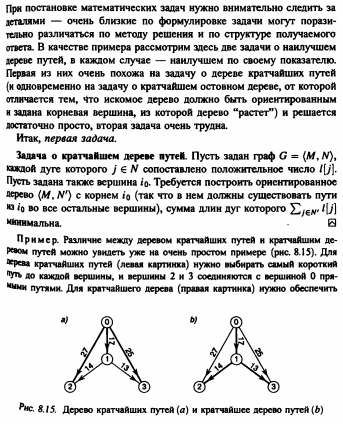
\includegraphics[width=10cm]{pics/47_1}
          \centering
  \end{figure}

  \begin{Alg}[двух китайцев] \
    \begin{figure}[H]
            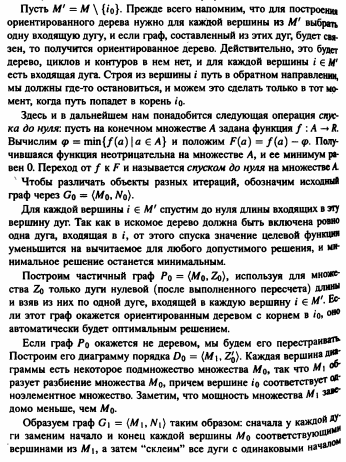
\includegraphics[width=10cm]{pics/47_2}
            \centering
    \end{figure}
    \begin{figure}[H]
            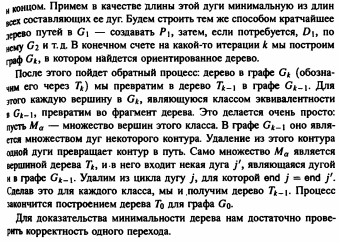
\includegraphics[width=10cm]{pics/47_3}
            \centering
    \end{figure}
  \end{Alg}

  \begin{figure}[H]
          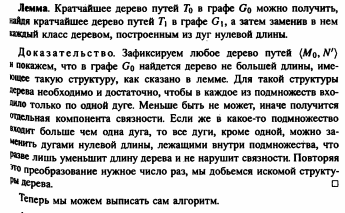
\includegraphics[width=10cm]{pics/47_4}
          \centering
  \end{figure}

  \begin{figure}[H]
          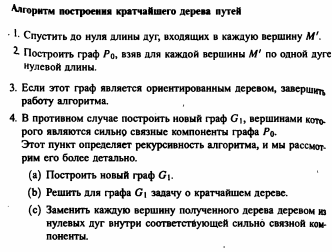
\includegraphics[width=10cm]{pics/47_5}
          \centering
  \end{figure}
\end{document}
